\documentclass[../th_cyber_warfare_distilled.tex]{subfiles}
 
\begin{document}

\chapter{หลักนิยมสงครามไซเบอร์}
\label{chapter:cyberwar_doctrine}
\section{ปฏิบัติการไซเบอร์}
ในปัจจุบันสหรัฐอเมริกายังไม่มีการกำหนดหลักนิยมสงครามไซเบอร์อย่างเป็นทางการแต่มีการประยุกต์ใช้แนวทางการรักษาความมั่นคงปลอดภัยระบบสารสนเทศและการสื่อสารจนกล่าวได้ว่าแนวทางดังกล่าวเป็นปฏิบัติการเชิงรับ โดยหากกระทำสำเร็จจะมั่นใจได้ว่าทรัพยากรที่เกี่ยวข้องกับข้อมูลข่าวสารทั้งปวงถูกสร้าง รับ-ส่ง ผ่านโครงสร้างพื้นฐานระบบสารสนเทศและการสื่อสารอย่างมั่นคงปลอดภัย และสามารถบริหารจัดการความเสี่ยงที่เกี่ยวข้องกับการโจมตีทางไซเบอร์ได้อย่างมีประสิทธิภาพ
\begin{figure}
	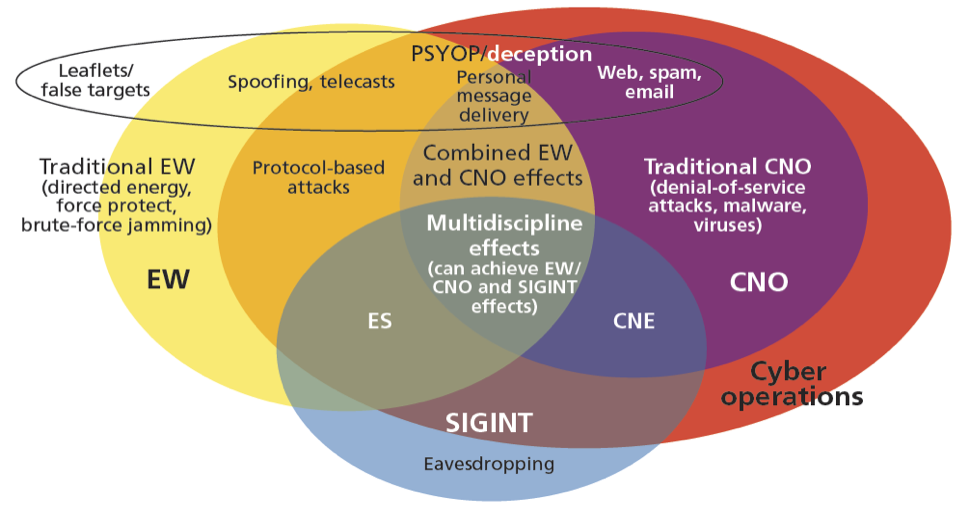
\includegraphics[scale=1]{figure_overall_io.png}
	\centering
	\caption{ภาพรวมการปฏิบัติการข้อมูลข่าวสาร}
	\label{figure:overall_io}
\end{figure}
สำหรับการปฏิบัติเชิงรุก สหรัฐอเมริกากำหนดแนวทางการปฏิบัติเกี่ยวกับสงครามไซเบอร์เป็นส่วนหนึ่งของปฏิบัติการข้อมูลข่าวสาร (IO) ดังแสดงในภาพที่ \ref{figure:overall_io} และเรียกปฏิบัติการที่เกี่ยวข้องกับสาขานี้ว่า ``ปฏิบัติการด้านเครือข่ายคอมพิวเตอร์ (Computer Network Operation)" ครอบคลุมถึงปฏิบัติการสาขาย่อยๆ 3 สาขาได้แก่
\begin{itemize}
	\item \textbf{การเจาะระบบเครือข่าย (Computer Network Exploitation)} หมายถึงกิจกรรมทั้งปวงที่หวังผลให้สามารถเข้าถึง และควบคุมทรัพยากรสารสนเทศของฝ่ายตรงข้ามได้ เช่นการเจาะระบบเครือข่าย การฝังโทรจัน การล่อลวงด้วยเทคนิคที่เกี่ยวข้องกับวิศวกรรมเชิงสังคม (Social Engineer) 
	\item \textbf{การโจมตีระบบเครือข่าย (Computer Network Attack)} หมายถึงกิจกรรมทั้งปวงที่กระทำขึ้นเพื่อทำลายทรัพยากรสารสนเทศของฝ่ายตรงข้ามให้ไม่สามารถใช้งานได้
	\item \textbf{การป้องกันระบบเครือข่าย (Computer Network Defense)}
	หมายถึงกิจกรรมทั้งปวงที่กระทำขึ้นเพื่อไม่ให้ฝ่ายตรงข้ามเข้าใช้ประโยชน์ทรัพยาการสารสนเทศของฝ่ายเรา
\end{itemize}

เมื่อพิจารณาภาพที่ \ref{figure:overall_io} จะเห็นว่าปฏิบัติการไซเบอร์ยังครอบคลุมถึงการดักรับดักฟังสัญญาณและคลื่นแม่เหล็กไฟฟ้า การปฏิบัติการจิตวิทยาและการลวง การปลอมแปลงสัญญาณ ตลอดจนการโจมตีต่อโพรโทคอลทางการสื่อสาร ดังนั้นหากต้องการป้องกันการโจมตีทางไซเบอร์จึงมีความจำเป็นอย่างยิ่งที่จะต้องจัดเสริมสร้างปัจจัยที่เกี่ยวข้องกับทรัพยากรสารสนเทศ 3 ปัจจัยหลัก ได้แก่
\begin{itemize}
	\item \textbf{ทรัพยากรมนุษย์ (People)} ได้แก่ บุคลากรต่างๆที่เกี่ยวข้องกับการวางแผนและการปฏิบัติการทางทหาร โดยบุคลากรเหล่านี้จะต้องมี ``ความตระหนักรู้" เกี่ยวกับความมั่นคงปลอดภัยที่เกี่ยวข้องกับการใช้งานทรัพยากรสารสนเทศทั้งปวงนับตั้งแต่กระบวนการสร้างข้อมูลข่าวสาร การปฏิบัติตามกฎระเบียบที่เกี่ยวข้องกับการรักษาความมั่นคงปลอดภัย การพัฒนาให้บุุคลากรมีทักษะและความรู้ที่เกี่ยวข้องกับปฏิบัติการ ฯลฯ
	\item \textbf{กระบวนการบริหารจัดการข้อมูลข่าวสาร (Process)} ได้แก่การกำหนดระเบียบวิธีปฏิบัติ ระเบียบปฏิบัติประจำที่เกี่ยวข้องกับการใช้งานระบบสารสนเทศและการสื่อสารอย่างมั่นคงปลอดภัย การเฝ้าตรวจความมั่นคงปลอดภัยของโครงสร้างพื้นฐานระบบสารสนเทศและการสื่อสาร การคัดเลือกและกำหนดสิทธิ์ในการเข้าถึงทรัพยากร ข้อกำหนดการเชื่อมต่อเครือข่าย ข้อกำหนดการพิสูจน์ตัวจริง ฯลฯ 
	\item \textbf{เทคโนโลยีสารสนเทศและการสื่อสาร (Technology)} ได้แก่การประยุกต์ใช้เทคโนโลยีสารสนเทศและการสื่อสารอย่างมั่นคงปลอดภัย เช่นการประยุกต์ใช้งานวิทยาการรหัสลับที่มีความมั่นคงปลอดภัยสูงในการเข้ารหัสข้อมูลที่มีความลับก่อนการับ-ส่งผ่านเครือข่าย การเข้ารหัสฮาร์ดดิสก์เพื่อป้องกันข้อมูลรั่วไหลหากเกิดการโจรกรรม เทคโนโลยีการประมวลผลข้อมูลขนาดมหึมาในการสร้าง Common Operational Picture ฯลฯ
\end{itemize} 

\begin{figure}
	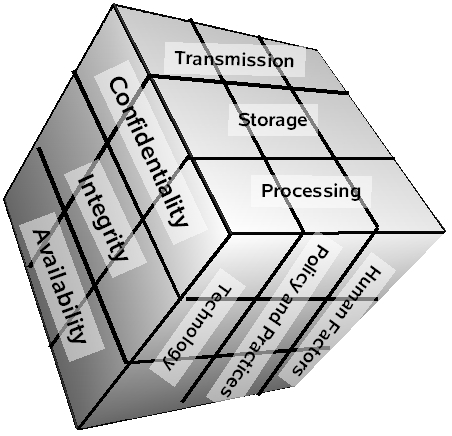
\includegraphics[scale=0.5]{figure_mccumber_cube.jpg}
	\centering
	\caption{แบบจำลองการรักษาความมั่นคงปลอดภัยของ J. McCumber}
	\label{figure:mcumber_cube}
\end{figure}

\section{หลักการรักษาความมั่นคงปลอดภัย}

ภาพที่ \ref{figure:mcumber_cube} แสดงแบบจำลองการรักษาความมั่นคงปลอดภัยทรัพยากรสารสนเทศของ J. McCumber ซึ่งแสดงองค์ประกอบที่จำเป็นในการรักษาความมั่นคงปลอดภัยใน 3 มิติคือ เป้าหมายหลักของการรักษาความมั่นคงปลอดภัย (desired goals) สถานะของสารสนเทศ (information state) และ แนวทางป้องกัน (safe guards)

\subsection{เป้าหมายหลักของการรักษาความมั่นคงปลอดภัย}
\begin{itemize}
	\item \textbf{การรักษาความลับ (Confidentiality)} หมายถึง การจัดการให้ทรัพยากรนั้นถูกล่วงรู้และแปลความหมายได้จากผู้ที่มีสิทธิ์ เช่นพาสเวิร์ดสำหรับการเข้าระบบควรเป็นสิ่งที่รู้เฉพาะบุคคล ข้อมูลระดับชั้นลับมากจะต้องไม่ถูกล่วงรู้จากผู้ที่ได้รับสิทธิ์เข้าถึงข้อมูลระดับชั้น ``ลับ" เป็นต้น
	\item \textbf{การรักษาความครบถ้วนสมบูรณ์ (Integrity)} หมายถึง การจัดการให้ทรัพยากรนั้นมีความครบถ้วนสมบูรณ์ มีกลไกตรวจสอบการถูกเปลี่ยนแปลงแก้ไข เช่นรายชื่อการแต่งตั้งดำรงตำแหน่งจะต้องไม่ถูกเปลี่ยนในขั้นตอนการนำเสนอผู้บังคับบัญชาจากผู้ไม่มีสิทธิ์โดยตรวจสอบไม่ได้ เป็นต้น
	\item \textbf{การรักษาความพร้อมใช้ (Availability)} หมายถึง การจัดการให้ทรัพยากรนั้นถูกเข้าถึงและใช้งานได้จากผู้มีสิทธิ์อยู่เสมอ เช่นระบบไฟฟ้าจะต้องพร้อมใช้งานไม่มีเหตุการณ์ไฟดับ ระบบบริการเว็บจะต้องพร้อมใช้งานในเวลาปฏิบัติราชการ เป็นต้น
\end{itemize}

\subsection{สถานะของทรัพยากรสารสนเทศ}
\begin{itemize}
	\item \textbf{การจัดเก็บ (Storage)} หมายถึง ทรัพยากรสารสนเทศใดๆที่ถูกจัดเก็บในแหล่งจัดเก็บข้อมูลเช่นสภาวะที่สารสนเทศนั้นถูกจัดเก็บในหน่วยความจำ ฮาร์ดดิสก์ การจัดเก็บเอกสารที่มีชั้นความลับที่มีการตรวจสอบการเข้าถึงห้องและมีการตรวจสอบสิทธิ์ เป็นต้น
	\item \textbf{การประมวลผล (Processing)} หมายถึง ทรัพยากรสารสนเทศใดๆที่ถูกกำลังถูกประมวลผล ทั้งในกระบวนการนอกระบบสารสนเทศและการสื่อสาร เช่นการพิมพ์ผลการทำ IPB แล้วทิ้งถังขยะโดยไม่มีการทำลายข้อความ ฯลฯ
	\item \textbf{การรับส่ง (Transmission)} หมายถึง ทรัพยากรสารสนเทศใดๆที่กำลังถูกรับ-ส่งผ่านตัวกลางการสื่อสาร เช่น การส่งข้อมูลพิสูจน์ตัวจริงผ่านเครือข่าย เป็นต้น
\end{itemize}

\subsection{แนวทางการป้องกัน}
\begin{itemize}
	\item \textbf{กระบวนการ (Process)} หมายถึง การกำหนดระเบียบ วิธีปฏิบัติที่เกี่ยวข้องกับการรักษาความมั่นคงปลอดภัยทรัพยากรสารสนเทศต่างๆ
	\item \textbf{ทรัพยากรมนุษย์ (People)} หมายถึง บุคคลที่มีส่วนเกี่ยวข้องกับทรัพยากรสารสนเทศ นั้นๆ
	\item \textbf{เทคโนโลยี (Technology)} หมายถึง เทคโนโลยีที่เกี่ยวข้องและสามารถนำมาประยุกต์ใช้ในการรักษาความมั่นคงปลอดภัยทรัพยากรสารสนเทศ เช่นเทคโนโลยีการเข้ารหัสลับ เทคโนโลยีที่เกี่ยวข้องกับการพิสูจน์ตัวจริง เป็นต้น
\end{itemize}

จากแบบจำลองนี้เมื่อต้องการรักษาความมั่นคงปลอดภัยให้กับทรัพยากรใดๆผู้มีส่วนเกี่ยวข้องจะต้องพิจารณาเป้าหมายหลักของการรักษาความมั่นคงปลอดภัยร่วมกับมุมมองอื่นๆคือสถานะของสารสนเทศ และแนวทางป้องกัน ยกตัวอย่างเช่นพื้นผิวที่เป็นจุดตัดกันระหว่าง การรับส่งข้อมูล การรักษาความลับ และเทคโนโลยี แสดงให้เห็นถึงความจำเป็นที่จะต้องมีการเลือกใช้เทคโนโลยีที่เหมาะสมสำหรับการรักษาความลับของข้อมูลข่าวสารที่ถูกรับส่งระหว่างกันซึ่งเทคโนโลยีที่เกี่ยวข้องในกรณีนี้อาจเกี่ยวข้องกับการเข้ารหัสข้อมูลข่าวสารนั้นๆ กระบวนการพิสูจน์ตัวจริงของอุปกรณ์สื่อสารเพื่อให้มั่นใจได้ว่าการรับส่งข้อมูลนั้นจะไม่ถูกส่งต่อไปยังอุปกรณ์ที่ไม่ได้รับสิทธิ์ ทั้งนี้แบบจำลองนี้จะถูกใช้ในการพิจารณากำหนดนโบยายและข้อกำหนดที่เกี่ยวข้องกับการควบคุม การประยุกต์ใช้งานเทคโนโลยีต่างๆเช่น วิทยาการรหัสลับ เทคโนโลยีโทรคมนาคม อย่างเหมาะสม
\end{document}